
%% Author_tex.tex
%% V1.0
%% 2012/13/12
%% developed by Techset
%%
%% This file describes the coding for rsproca.cls
\documentclass[PTRSB]{rsos}
\makeatletter\if@twocolumn\PassOptionsToPackage{switch}{lineno}\else\fi\makeatother

%Publisher: Royal Society
%Template Provided By: Typeset

\usepackage{amsmath,tabulary,graphicx,multicol}
\usepackage[utf8]{inputenc}
\long\def\ack#1{{\vskip5.5pt\noindent \fontsize{8}{11}\selectfont#1}}
\renewcommand{\neg}{{}^-}

%%%%%%%%%%%%%%%%%%%%%%%%%%%%%%%%%%%%%%%%%%%%%%%%%%%%%%%%%%%%%%%%%%%%%%%%%%
% Following additional macros are required to function some 
% functions which are not available in the class used.
%%%%%%%%%%%%%%%%%%%%%%%%%%%%%%%%%%%%%%%%%%%%%%%%%%%%%%%%%%%%%%%%%%%%%%%%%%
\usepackage{url,multirow,morefloats,floatflt,cancel,tfrupee}
\makeatletter


\AtBeginDocument{\@ifpackageloaded{textcomp}{}{\usepackage{textcomp}}}
\makeatother
\usepackage{colortbl}
\usepackage{xcolor}
\usepackage{pifont}
\usepackage[nointegrals]{wasysym}
\urlstyle{rm}
\makeatletter

%%%For Table column width calculation.
\def\mcWidth#1{\csname TY@F#1\endcsname+\tabcolsep}

%%Hacking center and right align for table
\def\cAlignHack{\rightskip\@flushglue\leftskip\@flushglue\parindent\z@\parfillskip\z@skip}
\def\rAlignHack{\rightskip\z@skip\leftskip\@flushglue \parindent\z@\parfillskip\z@skip}


\if@twocolumn\usepackage{dblfloatfix}\fi
\usepackage{ifxetex}
\ifxetex\else\if@twocolumn\usepackage{dblfloatfix}\fi\fi

\AtBeginDocument{
\expandafter\ifx\csname eqalign\endcsname\relax
\def\eqalign#1{\null\vcenter{\def\\{\cr}\openup\jot\m@th
  \ialign{\strut$\displaystyle{##}$\hfil&$\displaystyle{{}##}$\hfil
      \crcr#1\crcr}}\,}
\fi
}

%For fixing hardfail when unicode letters appear inside table with endfloat
\AtBeginDocument{%
  \@ifpackageloaded{endfloat}%
   {\renewcommand\efloat@iwrite[1]{\immediate\expandafter\protected@write\csname efloat@post#1\endcsname{}}}{}%
}%

\def\BreakURLText#1{\@tfor\brk@tempa:=#1\do{\brk@tempa\hskip0pt}}
\let\lt=<
\let\gt=>
\def\processVert{\ifmmode|\else\textbar\fi}
\let\processvert\processVert

\@ifundefined{subparagraph}{
\def\subparagraph{\@startsection{paragraph}{5}{2\parindent}{0ex plus 0.1ex minus 0.1ex}%
{0ex}{\normalfont\small\itshape}}%
}{}

%%% These are now gobbled, so won't appear in the PDF.
\newcommand\role[1]{\unskip}
\newcommand\aucollab[1]{\unskip}
  
\@ifundefined{tsGraphicsScaleX}{\gdef\tsGraphicsScaleX{1}}{}
\@ifundefined{tsGraphicsScaleY}{\gdef\tsGraphicsScaleY{.9}}{}
%%% To automatically resize figures to fit inside the text area
\def\checkGraphicsWidth{\ifdim\Gin@nat@width>\linewidth
	\tsGraphicsScaleX\linewidth\else\Gin@nat@width\fi}

\def\checkGraphicsHeight{\ifdim\Gin@nat@height>.9\textheight
	\tsGraphicsScaleY\textheight\else\Gin@nat@height\fi}

\def\fixFloatSize#1{}%\@ifundefined{processdelayedfloats}{\setbox0=\hbox{\includegraphics{#1}}\ifnum\wd0<\columnwidth\relax\renewenvironment{figure*}{\begin{figure*}}{\end{figure*}}\fi}{}}
\let\ts@includegraphics\includegraphics

\def\inlinegraphic[#1]#2{{\edef\@tempa{#1}\edef\baseline@shift{\ifx\@tempa\@empty0\else#1\fi}\edef\tempZ{\the\numexpr(\numexpr(\baseline@shift*\f@size/100))}\protect\raisebox{\tempZ pt}{\ts@includegraphics{#2}}}}

\renewcommand{\includegraphics}[1]{\ts@includegraphics[width=\checkGraphicsWidth]{#1}}
\AtBeginDocument{\def\includegraphics{\@ifnextchar[{\ts@includegraphics}{\ts@includegraphics[width=\checkGraphicsWidth,height=\checkGraphicsHeight,keepaspectratio]}}}

\def\URL#1#2{\@ifundefined{href}{#2}{\href{#1}{#2}}}

%%For url break
\def\UrlOrds{\do\*\do\-\do\~\do\'\do\"\do\-}%
\g@addto@macro{\UrlBreaks}{\UrlOrds}

\@ifundefined{quoteAttrib}
	{\long\def\quoteAttrib#1{\par\raggedleft\itshape#1\unskip}}
	{}

\@ifundefined{titlequoteAttrib}
	{\long\def\titlequoteAttrib#1{\list{}{\topsep-3pt\leftmargin.5in\rightmargin0pt}%
  \item\relax---\upshape#1\endlist}}{}

\renewenvironment{quote}
	{\list{}{\leftmargin.5in\rightmargin\leftmargin}%
  \item\relax}
  {\endlist}

\newenvironment{title-quote}
	{\list{}{\fontsize{10pt}{12pt}\selectfont\leftmargin.5in\itshape\rightmargin\leftmargin}%
  \item\relax}
  {\endlist}


\makeatother
\def\floatpagefraction{0.8} 
\def\dblfloatpagefraction{0.8}
\def\style#1#2{#2}
\def\xxxguillemotleft{\fontencoding{T1}\selectfont\guillemotleft}
\def\xxxguillemotright{\fontencoding{T1}\selectfont\guillemotright}
%%%%%%%%%%%%%%%%%%%%%%%%%%%%%%%%%%%%%%%%%%%%%%%%%%%%%%%%%%%%%%%%%%%%%%%%%%



\Journal{Phil.
Trans.
R.
Soc.
B }

%\usepackage[nolists,nomarkers]{endfloat}

%%%% Article title to be placed here
\title{Single-World Counterfactual Inference}

\author{%%%% Author details
Joshua Kaminsky$^{1}$, Lindsay T.
Keegan$^{1}$,\\C.
Jessica E.
Metcalf$^{12}$ and Justin Lessler$^{1}$}

%%%%%%%%% Insert author address here
\address{$^{1}$Department of Epidemiology, Johns Hopkins Bloomberg School of Public Health, Baltimore, MD, USA\\
$^{2}$Department of Ecology and Evolutionary Biology, Princeton University, Princeton, NJ, USA}

%%%% Subject entries to be placed here %%%%
\subject{Epidemiology, Infectious Disease Modeling}

%%%% Keyword entries to be placed here %%%%
\keywords{Counterfactuals, Infectious disease modeling, Infectious disease Dynamics, Network Modeling}

%%%% Insert corresponding author and its email address}
\corres{Justin Lessler\\
\email{justin@jhu.edu}}

\begin{document}
%%%% Abstract text to be placed here %%%%%%%%%%%%
% Recount words
\begin{abstract} % 197 words MAX 200 words
  Determining the effects of an intervention on a disease outbreak is an important problem in epidemiology. %15 words
  However, multiple confounders and sources of noise make it difficult to address. %12 words
  Here we present a method that addresses an important source of noise, stochastic variation of disease spread within the same population. %21 words
  Our method, like many others, employs compartmental models and extends an individual-level effect of the intervention to the population-level effect. %22 words
  We eliminate stochastic variation between epidemics by tracking both what happens with intervention and what happens without intervention within a single simulated epidemic. %23 words
  To simultaneously keep track of both states, we store all transition states that are possible either with or without the intervention on a network. %24 words
  We can actualize this network to recover the events that occur both with and without the intervention. %17 words
  We demonstrate our method by estimating cases averted by four interventions during an influenza-like illness outbreak. % 17 words
  We find that our method reduces the variance of all estimates, and in one case makes the results statistically significant. %20 words
  Although our method is more computationally intensive than traditional methods, it is computationally tractable for many common use cases, making it a useful tool for selecting interventions. %26 words
\end{abstract}
%%%%%%%%%%%%%%%%%%%%%%%%%%%


%%%%%%%%%%%%%%% End of first page %%%%%%%%%%%%%%%%%%%%%

\maketitle

\begin{multicols}{2}
\section{Introduction}
Dynamic models are frequently used to assess the likely impact of disease control strategies.
These exercises range from modeling the impact of a new intervention or strategy on an established pathogen [MORE CITATIONS] \cite{ferguson-et-al:2005,azman-et-al:2016}, to models of the containment and control of emergent epidemics [MORE CITATIONS] \cite{lessler-et-al:2016}.
While deterministic models are frequently used \cite{meltzer-et-al:2014,dodd-et-all:2010,fraser-et-al:2004}, stochastic simulations are increasingly common as they can account for both uncertainty in the underlying parameters and the random nature of the disease process [MULTIPLE CITATIONS]\cite{ferguson-et-al:2003}.
In both stochastic and deterministic models, the impact of interventions are typically determined by comparison of simulations with and without the intervention.

In the deterministic setting, this comparison is straight forward, as with a given set of parameters and starting conditions the epidemic will always behave exactly the same; hence any comparison between an intervention scenario and its non-intervention `counterfactual' can only be attributed to the intervention itself.
When stochastic models are used, things become more complicated.
Typically, two sets of simulations are conducted, one with the intervention and one without, and then the distribution of outcomes from the two sets are compared to estimate the intervention effect.
Because these are independent sets of simulations, there may be some simulations in the non-intervention scenario where the disease dies off quickly due to random chance, and fewer cases occur than the majority of intervention simulations.
Likewise, there may be cases in the intervention scenario where large numbers are infected through sheer `bad luck' for the virtual populations involved.
If these stochastic effects are large, they may lead uncertainty intervals in effect estimates to include the intervention having no effect, or even a negative impact, even if the intervention is modeled in such a way that it can only have a beneficial effect.
For example, the results of a study of measles vaccination strategies by Lessler et al.
appears to leave open the possibility that more cases of measles could occur in a country if supplementary vaccination activities were conducted than if those campaigns had not occurred \cite{lessler-et-al:2016}.
Likewise, Rivers et al. is consistent with low coverage of pharmaceuticals causing additional cases of Ebola when compared to no coverage, even though the model assumes they have an effect \cite{rivers-et-al:2014}.
These effects will be exacerbated if the processes being modeled are complex or we are simultaneously sampling over parameter uncertainty.

The results of this independent simulation approach have a very specific interpretation: they represent the difference between what we expect to be observed in an uncontrolled epidemic compared to a completely independent epidemic where the intervention occurred (conditional on the starting conditions).
However, what we often want to know is what would have happen had the intervention occurred in the exact same epidemic.
This is equivalent to the problem of counterfactual inference in randomized trials and observational studies, where we take one set of individuals (or populations) as a stand in for what would have happened in the counterfactual situation that they had experienced some exposure.
A number of techniques of trial design and statistical analysis have been developed to help such real world studies better approximate the true counterfactual situation (\cite{hudgens-halloran:2008,murray-et-al:2017,buchanan:2014} are just a few examples of the large literature on the subject).
However, in computational simulations it is possible to take a more exact approach.

Here, we present a method for simulation of direct counterfactuals to stochastic simulations using principles borrowed from the percolation approach to epidemic simulation \cite{miller-book}.
We illustrate this `single-world' approach using simulations of interventions against an influenza like illness, and outline how the general approach can be adapted to a wide variety of disease systems and simulation methodologies.

\section{Methods}

\subsection*{Overall Approach}
Our goal is to simulate an uncontrolled epidemic and then simulate one or more controlled epidemics that are $100\%$ consistent with the uncontrolled epidemic.
That is, all events (e.g., transmissions, recoveries, etc.) that occur in the uncontrolled epidemic also occur in its controlled counterpart unless precluded (directly or indirectly) by the intervention; and no stochastic events that were possible in the uncontrolled epidemic occur in its controlled counterpart, unless explicitly caused by an intervention.
To accomplish this, we take an approach that first prunes events according to a model based stochastic simulation to create a `potential epidemic graph' (PEG) (Figure \ref{fig:pruning}) , and then use this graph to `realize' consistent epidemics in controlled and uncontrolled scenarios (Figure \ref{fig:actualizing}).

Specifically, our approach begins with an implicit set of all possible events, which we think of as a large graph where each edge is an event, and each node is a person at a time.
We call this graph the complete graph.
Events (i.e., directed edges) in the graph connect a node at one time step (the source), to a node in the next time step (the target) and have an \emph{outcome}, \emph{conditions}, and a \emph{probability}.
The target can be another individual (e.g., for transmission events) or the same individual (e.g., for recovery events).
Each event changes the state of its target, and we call the new state the \emph{outcome} (e.g., `immune' is the outcome of a recovery event).
Each event can only occur if both the state of its source and the state of its target at the previous time step meet certain \emph{conditions} (e.g., the source must be infectious and the target susceptible for a transmission event to occur).
The underlying epidemic model assigns each event a \emph{probability} of occurring if its conditions are met.
In the complete graph, each node is considered to potentially belong to any of a set of \emph{potential states} (e.g., susceptible, infectious, immune).

%Come back to this later: (i.e., remove those states that could only exist...)
As illustrated in Figure \ref{fig:pruning}, to create the PEG, we first assign individuals an initial state at time $0$ (equivalent to removing all but one of their potential states).
We then prune from the complete graph all of the edges whose conditions are inconsistent with the remaining potential states of each node.
Next, we stochastically prune the remaining edges based on their probability.
We then remove all states at time $1$ that are inconsistent with the remaining edges (i.e., remove those states that could only exist if an edge was added to the graph).
This process is then repeated iteratively until a predefined time limit is reached.

Once the PEG is created, an uncontrolled epidemic can be realized by iterating through times assuming all events whose conditions are met occur and setting each event's target node to the outcome of that event (Figure \ref{fig:actualizing}).
To simulate an intervention, the same process is performed, but edges are removed or node states changed probabilistically based on the intervention process.

Below, we provide a more detailed description of how to perform this process for epidemic systems specified by a compartmental model.

\subsection*{General Framework}
We define a general compartmental model as a system of difference equations with $K$ compartments governed by 
\begin{align*}
\Delta x_{j} &= \sum_{i \neq j} \alpha_{i,j}x_i + \sum_{i \neq j, k} \alpha_{i,j,k} x_ix_k.
\end{align*}
%% RETURN
At times, we may use $\alpha$ to refer to an $\alpha_{i,j,k}$ or an $\alpha_{i,j}$.
Each $\alpha_{i,j} > 0$ and $\alpha_{i,j,k} > 0$ represents the probability of one class of events and define the outcome and conditions of each event in that class.
We will sometimes say call refer to events by class: $\alpha_{i,j,k}$-events or $\alpha_{i,j}$-events.
The outcome of an $\alpha_{i,j,k}$-event or an $\alpha_{i,j}$-event is $j$.
$\alpha_{i,j}$-events require the source to be in state $i$, while $\alpha_{i,j,k}$-events require the source to be in state $i$ and the target to be in state $k$.
$\alpha_{i,j}$-events have the same person as their source and target, while $\alpha_{i,j,k}$-events have different sources and targets.
To construct the complete graph, we connect every person to themselves at the next time with an $\alpha_{i,j}$-event for each positive $\alpha_{i,j}$ and connect every person to each other person at the next time with an $\alpha_{i,j,k}$-event.
In the complete graph, each node has each of the $K$ compartments as potential states.

To construct the PEG, we take the complete graph, and alter the potential states of each node at $t_0$ according to our initial conditions.
We then prune the graph by applying three steps at each time: we prune events with conditions we know cannot be satisfied; we stochastically prune the remaining events according to their probability; and we eliminate potential states from the nodes according to our assumptions detailed below (Figure \ref{fig:pruning}).

%% Prune inconsistent events
Once we have information about the potential states of each person a time, then we can eliminate events inconsistent with those potential states.
If we know that $n$ is not in the potential states of a node at that time, then we prune any $\alpha_{i,j,n}$-events whose source is that node, any $\alpha_{n,j}$-events whose source is that node, and any $\alpha_{n,j,k}$-events whose target is that person at the next time.
We can repeat this process for each potential state, removing appropriate events from each node that does not have that state in their potential states.%Super double negativey

%% Prune according to probability
After pruning inconsistent events, we probabilistically test the remaining events according to their probability, removing each $\alpha_{i,j}$-event with probability $1-\alpha_{i,j}$ and each $\alpha_{i,j,k}$-event with probability $1-\alpha_{i,j,k}$.
We note here that in order for this process to work, we require that $\alpha_{i,j,k},\alpha_{i,j} \leq 1$.
This pruning step represents the main transition between the complete graph and the PEG: the events remaining after this step are not just possible, but will occur if their conditions are met.

%% Update Node states
We permit interventions to alter the course of the epidemic in two ways: interventions may remove $\alpha_{i,j,k}$-events, interventions may change the state of an node so long as that state change would not have added the events to the PEG.
These assumptions allow us to construct the PEG assuming that the potential states are determined by the events in the PEG at the previous time and any events since then.
For each state $n$, there are two ways for $n$ to be a potential state of a node: an event could change that person's state, or that person could remain in the state from the previous time.
A person potentially enters a state $n$ if they are the target of an edge with outcome $n$.
A person potentially remains in a state $n$ if their potential states at the last time include $n$, and no $\alpha_{n,j}$-edge has them as its target.
If that person was previously in state $n$, but an $\alpha_{n,j}$-edge has them as its target, then they would have become state $j$ instead of remaining in state $n$; and because we assume the intervention did not remove the $\alpha_{n,j}$-edge they did not remain in state $n$ for any intervention.
The same argument does not hold for an $\alpha_{n,j,k}$-edge, because the intervention could remove the event, which would result in the person remaining in state $j$.
A node's potential states are the states that it potentially remained in or that it potentially entered.

Now that we have constructed our PEG, we `realize' it using a control strategy (for uncontrolled epidemics, we use a null control strategy).
To `realize' the PEG, we prune it iterating three steps at each time: we prune events whose conditions are not met; we stochastically determine if the intervention removes any events; and we set actual state of each node allowing the intervention to alter the actual state (Figure \ref{fig:actualizing}).
The intervention plays two roles in this process, both preventing some events from happening in the second step, and altering the states of individuals directly in the third step.
When altering the states of individuals, we need to ensure we adhere to the assumptions set up in the previous paragraph.
The resulting graph has the actual state of each person at each time as well as all events that occurred, which allows us to extract most quantities of interest including both the normal SIR results (case counts at each time), and a transmission tree.

%% FIGURE 1
\begin{figure*}[hp]
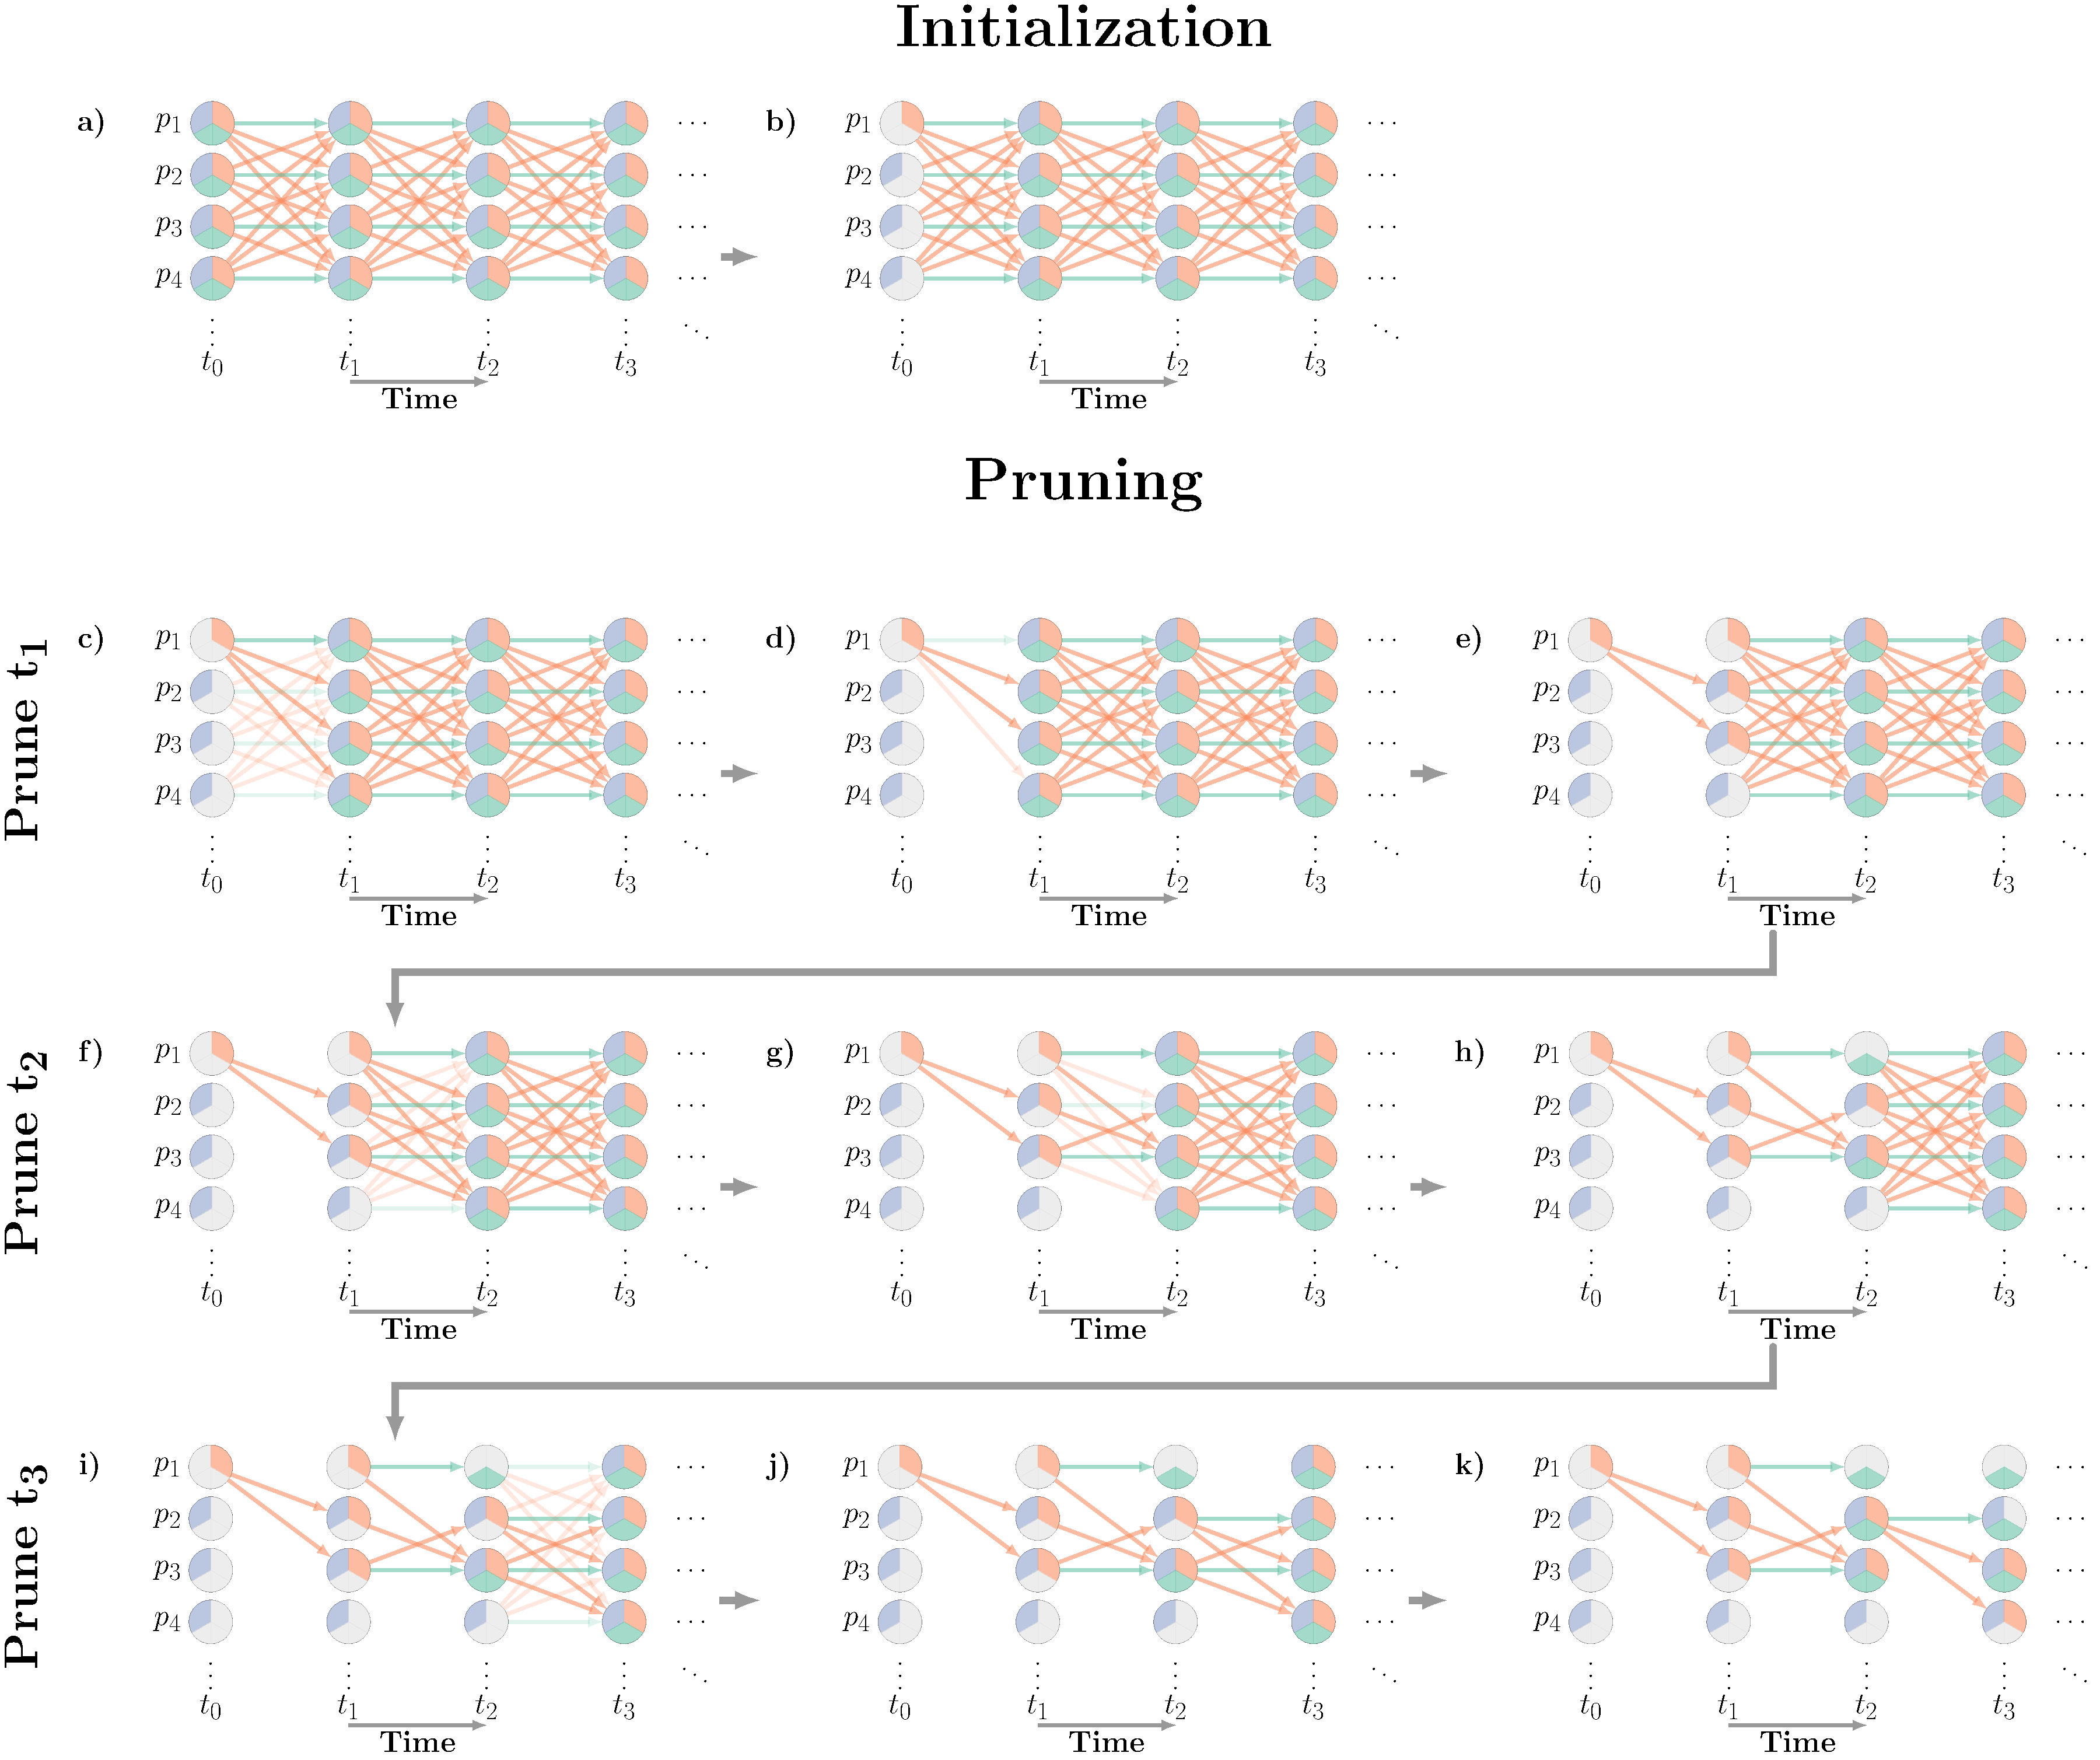
\includegraphics[width=\textwidth]{../figures/peg_create.pdf}
\caption{\textit{‘Single-world’ simulation process.}
  To simulate an initial epidemic and interventions, we start with a (implicit) graph where each node represents the possible states a person at particular time in the epidemic and edges represent possible events that can change a nodes state (a).
  In the above example, a person $p_i$ can be susceptible (purple pie slice), infectious (orange) or immune (green), and the possible events are transmission (orange arrows) and recovery (green arrows).
  We start by assigning each individual in the population a state at time $t_0$ (b), here infecting $p_1$.
  We next remove all edges with conditions we know are not satisfied based on the initial state (c).
  We then prune those edges stochastically selected not to occur by our underlying infection model (d).
  The possible states of each person at $t_1$ based on the edges still existing in the graph, so each person’s set of potential states encompasses those that could exist if each of the previous set of events did or did not exist (e).
  We now repeat steps c-e for events between $t_0$ and $t_1$ (f-h), $t_1$ and $t_2$ times 2 and 3 (i-k) and so on.
  Note that when we prune the edges with unattainable conditions, (i) we still keep the those for $p_1$ and $p_2$ infecting $p_3$, even though $p_3$ was potentially infected at $t_1$, because susceptibility is still a possible state for $p_3$ at $t_2$ in an intervention scenario (i.e., removing the transmission event at $t_1$ could lead to a scenario where $p_3$ is susceptible at $t_2$.)
  This final potential epidemic graph (PEG) can then be used to obtain simulated epidemics with and without interventions (see Figure \ref{fig:actualizing}).
}
\label{fig:pruning}
\end{figure*}

%% FIGURE 2
\begin{figure*}[hp]
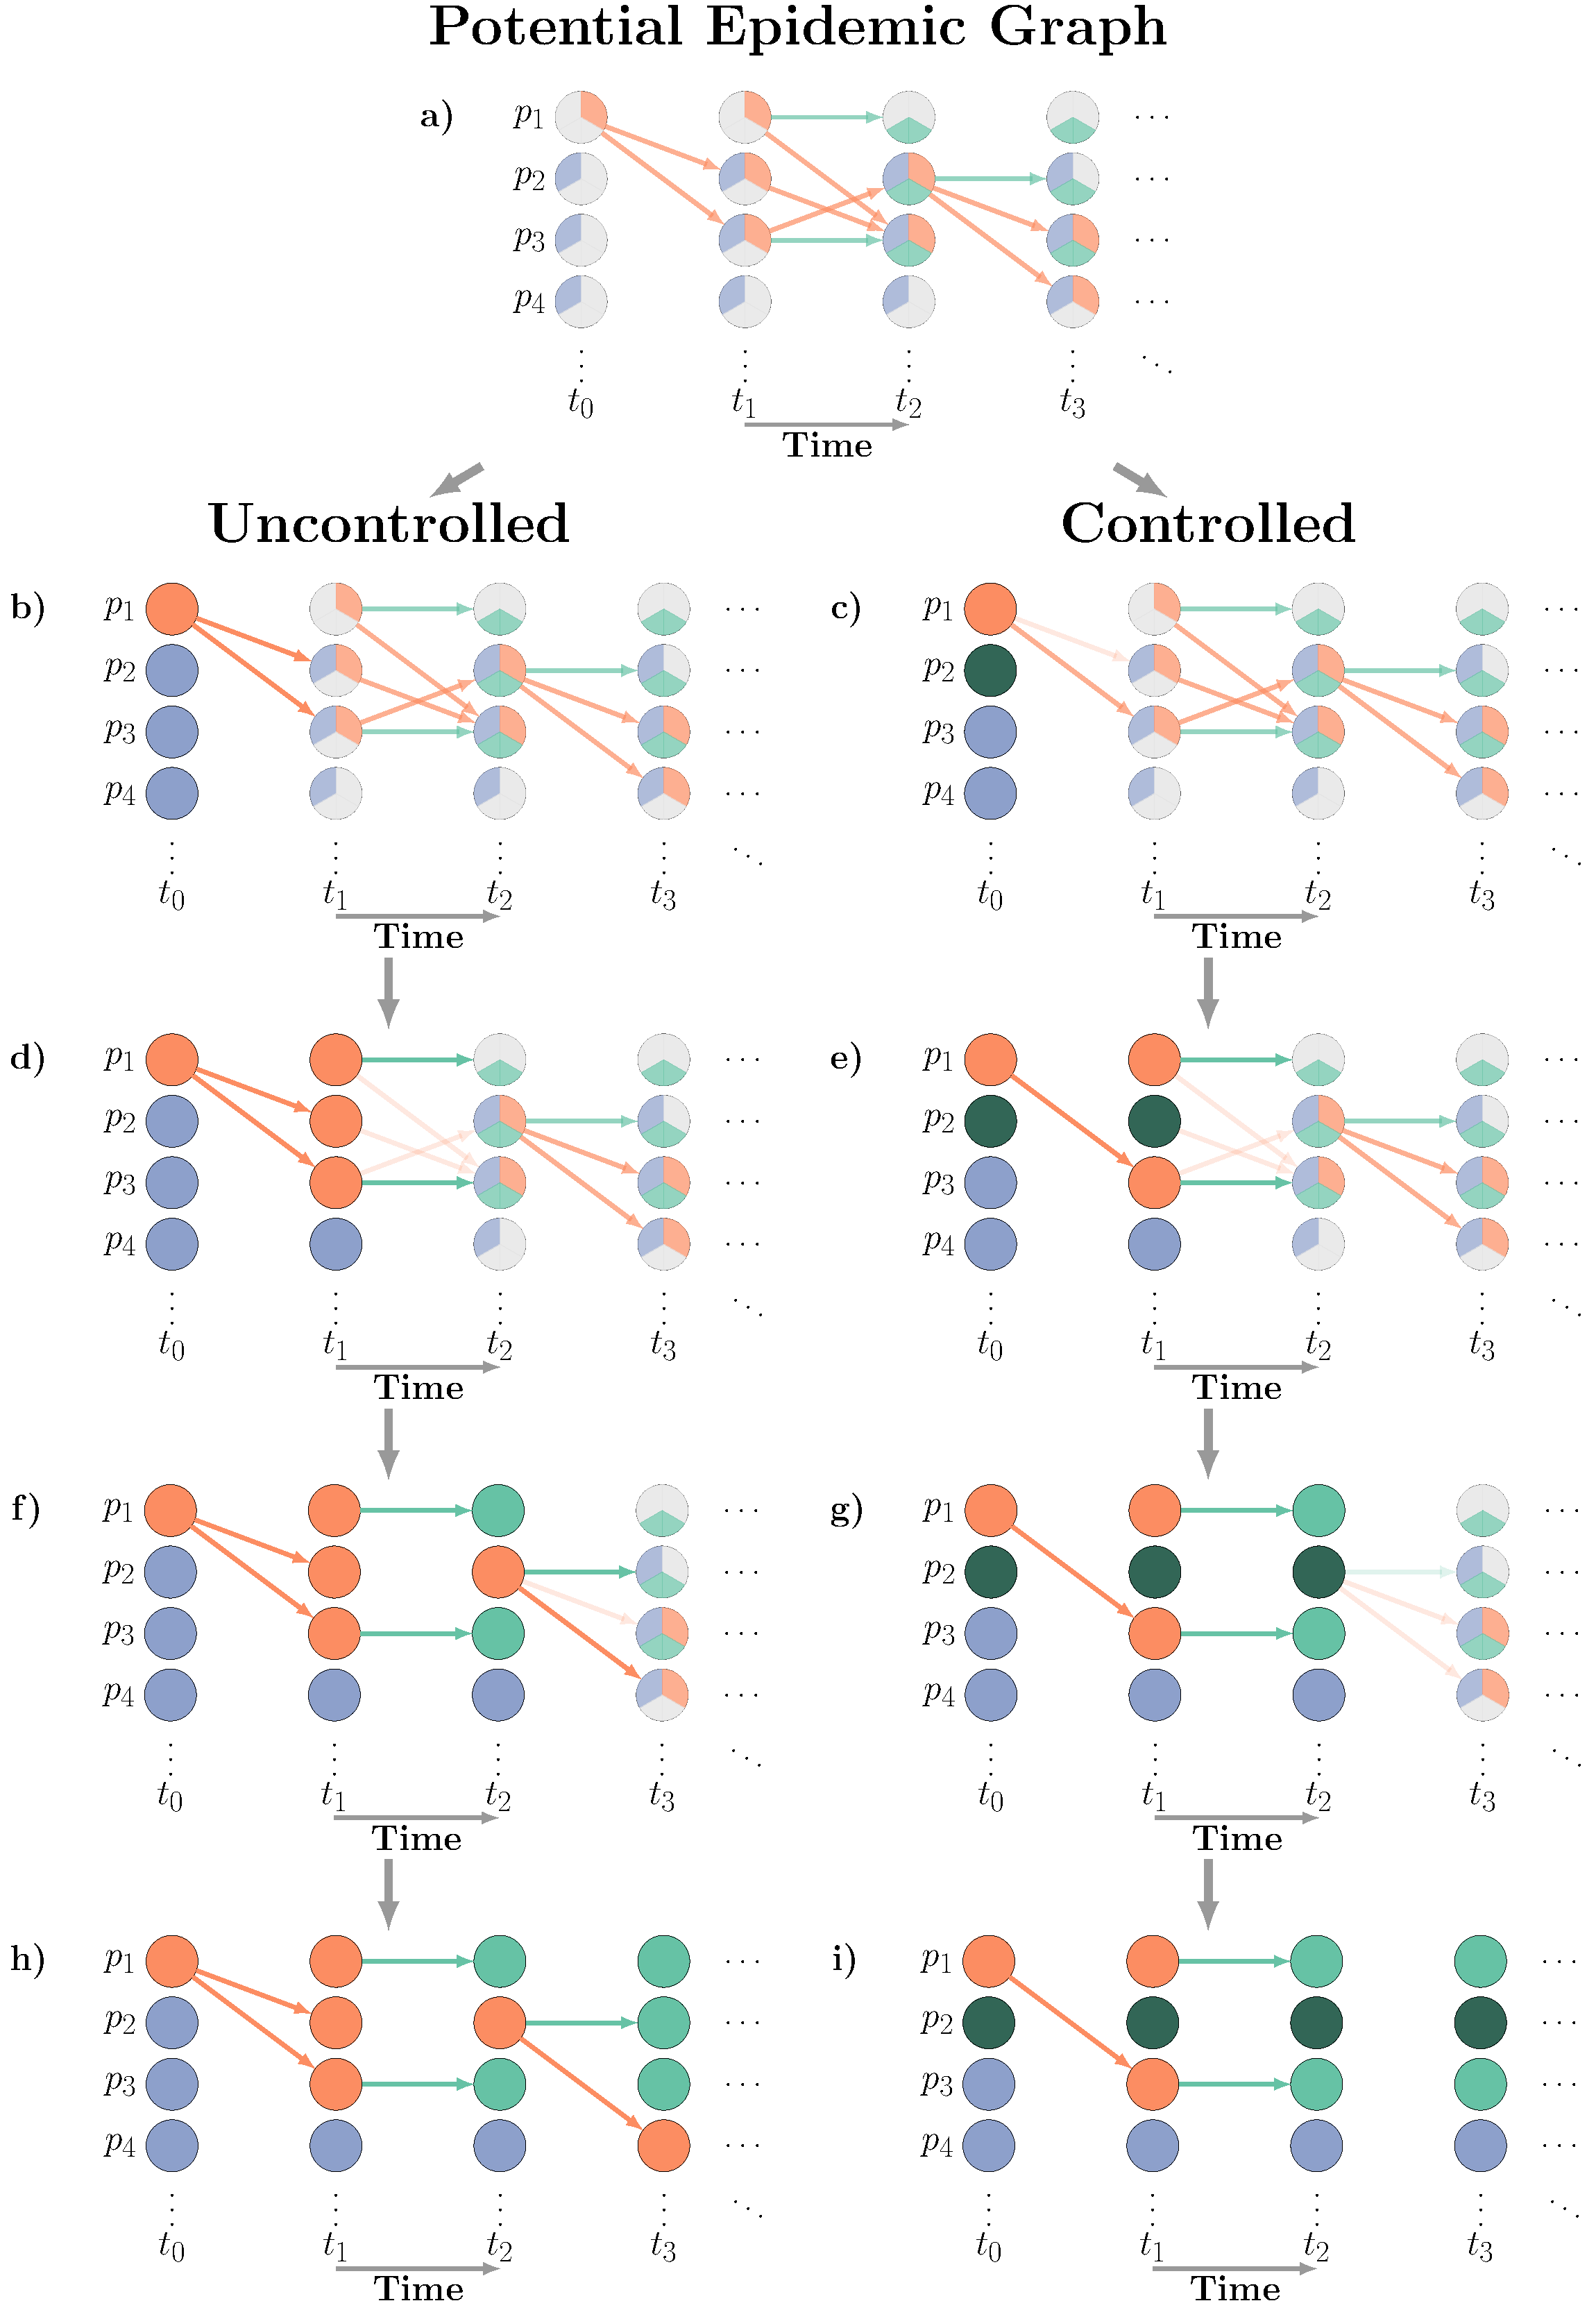
\includegraphics[width=\textwidth]{../figures/epidemic_both.pdf}
\caption{\textit{‘Single-world’ simulation process (continued).}
  To obtain simulated epidemics, we start with a potential epidemic graph (a) (see Figure \ref{fig:pruning} for how to create a epidemic potential graph (PEG)).
  In the above example, a person can be susceptible (purple pie slice), infectious (orange) or immune (green), and the possible events are transmission (orange arrows) and recovery (green arrows).
  %Potentially remove this
  In order to measure the impact of the intervention on the epidemic, we will use the potential epidemic graph to construct two epidemics: one uncontrolled (left) one with intervention (right).
  We start by setting the actual state of each person at time $t_0$ to their initial condition, and then allowing the change their initial states, in this case setting $p_2$ as vaccinated (dark green) (b,c).
  We then prune edges between $t_0$ and $t_1$: removing inconsistent edges and allowing the intervention to stochastically remove edges.
  We then use those edges to determine the actual state of each person at $t_1$ (d,e).
  We repeat the process for times $t_2$ (f,g), $t_3$ (h,i), and so on.
  This final graph can be used to extract our outcome of interest.
  Any graphs made from the same PEG represent the results of different interventions in a `single-world'.
}
\label{fig:actualizing}
\end{figure*}

\subsection*{Influenza Example}
To demonstrate our proposed method, we construct an influenza example using a standard Susceptible (S), Infected (I), Immune (R) compartmental model.
By modeling influenza transmission within a single season we do not account for loss of immunity and we assume that births and deaths are negligible.
We allow the probability of an infectious contact between any particular susceptible-infected pair to be $\beta = 0.78$ per day and the probability of an infected individual recovering at any time step to be $\gamma = 0.44$ per day \cite{forsberg-white-et-al:2009}.

We evaluate the effects of four control measures on influenza cases averted: hand-washing, vaccination, antivirals, and a null intervention.
We selected these example interventions to highlight different ways in which interventions can interact with the epidemiology.
We assume hand-washing reduces transmissibility by $1\%$, and therefore model it by removing $1\%$ of transmission events.
For vaccination, we chose $8.25\%$ of people to be fully vaccinated against influenza, and therefore begin as Vaccinated instead of Susceptible.
For the antiviral intervention, we choose $25\%$ of people to take antivirals when they first become infected, assume that it reduces their average duration of infection by $0.7$ days \cite{oseltamivir:2014}.
We model this by choosing $25\%$ of people at the start of the epidemic, and if they become infected, they have a $36.1\%$ additional chance to recover at each time step.
To highlight the differences between our method and traditional methods, we include a null intervention in which we do not intervene.
While this is not an intervention, it effectively demonstrates the ability of our method to reduce the process model variance.
We run $1,000$ simulations of each type of inference, for each intervention, on a population of $4,000$ for $100$ days and calculate the estimated number of cases averted.

\section{Results}

%% TABLE 1
\begin{table}
\caption{Space and time complexity results for our proposed method, with and without pruning, each step of our proposed method, and the current standard method.}
\begin{tabular}{|l|l|l|}
  \hline
  Task & Space Use & Time / simulation\\\hline
  %Construct Epidemic Potential Graph without pruning & $58.4$ TB & \textemdash \\\hline
  Construct Epidemic Potential Graph& $1.73$ GB & 54 seconds \\\hline
  Construct Realized Epidemic Graph& $1.3-1.4$ KB & $16-20$ seconds \\\hline
  Multiple-World Inference& $1.3-1.4$ KB &  $22-24$ seconds\\\hline
\end{tabular}
\label{table:performance}
\end{table}

%% FIGURE 4
\begin{figure*}
\centering
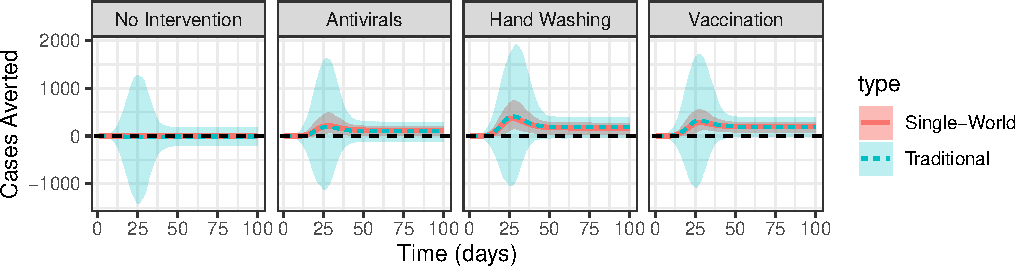
\includegraphics[width=\textwidth]{../figures/intervention-effects-time-series-cases-averted-switched-cropped.pdf}
\caption{Time series showing the number of cases averted at each time caused by the intervention calculated using our method (single-world) and a standard method (multiple-world).
 Of particular note, both methods produce the same point estimates (solid lines), but have different $95\%$ confidence intervals.
 The single-world method is consistently above $0$, while the multiple-world method tends to fall below $0$, particularly near the peak of the epidemic.
 At all times, the single-world method produces tighter confidence intervals than the multiple-world method.}
\label{fig:epicurve}
\end{figure*}

We evaluate the effects of four control measures on influenza cases averted: hand-washing, vaccination, antivirals, and a null intervention by running $1000$ trials on a population of $4000$ over $100$ days using both our proposed method and the current standard method.
We find that the two methods obtain the same general point estimates, but our method has narrower confidence intervals and avoids the nonsensical results of the other method (Figure \ref{fig:epicurve}).
We find that the our method takes about twice as much time as the standard methods for a single intervention, but with each additional intervention our method adds the same amount of time as the standard method (Table \ref{table:performance}).

For single-world inference, we found that every non-null intervention had a significant ($p<0.05$) number of cases averted: Null $ 0 $ (CI $ 0 $ \textemdash $ 0 $), Antivirals $ 632 $ (CI $ 318 $ \textemdash $ 2806 $), Social Distancing $ 152 $ (CI $ 9 $ \textemdash $ 295 $), Vaccination $ 284 $ (CI $ 149 $ \textemdash $ 431 $).
For multiple-world inference, we found that all but one non-null intervention had a significant ($p<0.05$) number of cases averted: Null $ \neg5 $ (CI $ \neg196 $ \textemdash $ 184 $), Antivirals $ 627 $ (CI $ 292 $ \textemdash $ 2808 $), Social Distancing $ 147 $ (CI $ \neg67 $ \textemdash $ 354 $), Vaccination $ 280 $ (CI $ 82 $ \textemdash $ 495 $).
In addition to estimates of cases averted, we observe that multiple-world has an unintuitive effect on the shape of the epidemic (Figure \ref{fig:epicurve}).

We released a software package, \texttt{counterfactual}, on \texttt{CRAN}, %NOTE: This is not true yet
which implements our method.
It follows the assumptions and procedures outlined above, but while it employs the intervention assumptions, it does not enforce them.
Time calculations for our method were made using this package.

\section{Discussion}
In this paper, we present a method that reduces uncertainty in estimates of the effects of control strategies by asking a refined counterfactual question.
We demonstrate the ability of our method to factor away cross-epidemic variation, which can lead to counterintuitive results.
Additionally, our method is tractable when applied to a broad class of models and interventions, simultaneously: many of which are supported by our software package.

Our method acheives these results by addressing a different question than most simulation-based methods: traditional methods ask how control would alter the number of cases in two independent epidemics in the same population; our method asks how control would alter the number of cases in a single epidemic.
Traditional methods are better suited to answer epidemic focused policy questions (e.g., How will an epidemic next year look if we implement control?), while our method is better suited for control focused questions, (e.g., How much better does ring vaccination perform than regular vaccination?).

Even when asking this different question, single-world inference has some inherent limitations.
Discrete time compartmental models are not cutting edge modeling techniques, and there are multiple generalizations we may want to use: continuous time models, network models, and agent-based models are all generalizations of compartmental models not covered by our method.
Moreover, some models are beyond the scope of this method for computational reasons: models with large numbers of compartments (e.g., metapopulation models) may not be tractable for large populations.
Some interventions are incompatible with the pruning assumptions: interventions which create new non-trivial compartments (e.g., temporary quarantine) and those that move people between compartments (e.g., forced migration) are incompatible with pruning.
Worse, even if we ignore tractability some interventions are beyond the scope of this method; an intervention may be so radical we cannot express it in a way the potential epidemic network captures.

Going forward, there is still interesting work to improve the tractability of the method both by optimizing computation and by examining our pruning assumptions.
Currently, the pruning assumptions are absolute, but stochastic assumptions may allow us to relax pruning assumptions and admit more control strategies.
We also hope to extend this method to apply to real-world epidemic data, answering questions about how potential interventions would have affected an epidemic that already occurred.
This method also serves as an example of marshalling computational resources to more precisely target our simulations, rather than running more simulations or simulating at a finer scale.

%Find me a home
We are not the first group to answer the refined counterfactual question: Kenah and Miller use percolation to measure the effects of a single intervention \cite{kenah-miller:2011}.
\enlargethispage{20pt}

\ethics{This research did not require ethics approval as it used simulated  data.}

\dataccess{Code used for the included analyses are available upon publication.}

\aucontribute{Conception and design of study: JL\\
Development and/or verification of analytic methods: JK and JL\\
Analysis and/or interpretation of results: JK, LTK, and JL\\
Drafting the manuscript: JK and LTK\\
Revising the manuscript: JK, LTK, CJM, and JL \\
Approval of the final manuscript: JK, LTK, CJM, and JL}

\competing{We have no competing interests.}

\funding{Insert funding text here.}

\ack{Insert acknowledgment text here.}
\end{multicols}

\bibliographystyle{RS}
\begin{multicols}{3}
\bibliography{bibliography}
\end{multicols}
\end{document}

%% Stuff for supplement
At this stage, we also need to account for the possibility of two conflicting events occuring (e.g., a person may become infected and grow older in an age cohort model).
In some cases the events interact (the person grows older and is infected), in other cases one event takes precedence over the other (a person who dies and gets infected is dead).
It is up to the modeler to account for these cases, and determine what should happen.

The amount of space and time pruning takes in the software package is $\mathcal O(E)$, where $E[O(E)] = O(t(n^2\sum \alpha_{i,j,k} + n \sum\alpha_{i,j}))$ per simulation, or $O(t(n^2\beta + n\gamma))$ in the case of the SIR model.
The amount of time the interventions take is also $\mathcal O(E)$, but the constant is lower (Table \ref{table:performance}).
This shows us that the number of infectious compartments, the population, number of times, and number of simulations all impact the amount of time taken, but population has the biggest impact.

%% FIGURE 3
\begin{figure*}
\centering
\includegraphics[width=.31\textwidth]{../figures/intervention-effects-raw-boxplots-cropped}
\includegraphics[width=.31\textwidth]{../figures/intervention-effects-combined-boxplots-cropped}
\caption{\textbf{Left)} \textbf{Boxplots of simulations results under the each intervention scenario.}  Notice that all of the boxplots overlap, which implies that from the population perspective, the effects of the interventions are all insignificant.
 \textbf{Right)} The single-world estimate of cases averted for each intervention scenario.
 Unlike the right hand figure, very few of the boxplots overlap with The null intervention.}
\label{fig:boxplots}
\end{figure*}

